% BP
% 1.项目概况
% 2.产品及服务
% 3.行业竞争及市场渠道
% 4.技术特点和核心竞争力
% 5.团队介绍
% 6.融资计划和未来规划

% 商业计划书要素提示
% 01.公司概况
% 公司的成立背景及历史沿革、公司的主要产品/服务及业务发展状况、公司发展的里程碑或大事记等。(让阅读者对公司的关键信息有初步了解)
% 02.市场分析
% 市场细分及市场定位、用户购买特征及关键购买因素、市场规模及增长率等。
% 03.产品(服务)
% 核心技术、产品研发策略等。
% 04.营销策略
% 产品的价格策略、渠道策略、市场推广策略等。
% 05.竞争分析
% 对行业的分析、对国内外主要竞争对手的分析、对自身的分析和竞争策略等。
% 06.业务模式
% 价值定位分析(能给用户带来怎样的使用价值,解决用户的哪些关键需求)、产业价值链分析(根据本行业特征做行业价值链分析)、价值链定位及组合(公司选择做价值链的哪些环节并形成怎样的组合)、收入模式分析等。
% 07.业务发展状况
% 在技术/产品研发方面取得的成绩、在市场拓展方面取得的成绩等。
% 08.公司股权结构
% 公司的股权结构及历次变更情况、公司股东的背景情况及对股东的评价等。
% 09.公司治理结构
% 公司股东会和董事会的组成、公司股东会和董事会的运作状况、管理者对股东会和董事会的评价等。
% 10.管理团队
% 管理团队主要成员的简历、对管理团队成员的评价等。
% 11.公司组织结构
% 公司的组织结构及职能分工、公司组织运作的基本状况及评价等。
% 12.公司战略规划
% 公司的宗旨与使命、价值观与核心理念、近期/中期/远期目标、发展策略及实施步骤、三年内的业务规划等。
% 13.融资计划
% 公司的融资规模及准备出让的股权比例、资金使用计划、对投资人的退出计划等。
% 14.财务分析
% 公司的历史财务报表、未来三年的财务预测、公司的价值评估、投资人可能获得的收益预测等。
% 15.风险分析
% 市场风险、产品/技术风险、经营风险、管理风险、财务风险等。
% 16.其它信息
% 创业者认为需要披露的对投资人有价值的信息。
\documentclass[a4paper,11pt]{article}
\usepackage[margin=1in]{geometry}
\usepackage{xeCJK}
\defaultCJKfontfeatures{Scale=1.1}
\setCJKmainfont{SourceHanSerifCN-Regular}
\setCJKmonofont{SourceHanSerifCN-Regular}
\setmainfont{SourceHanSerifCN-Regular}
\renewcommand{\baselinestretch}{1.7}
\usepackage{graphicx}       % front image
\usepackage{caption}
\usepackage{subcaption}
\usepackage{hyperref}       % links and email
\usepackage[english]{babel} % linebreaks for english words
\usepackage{eurosym}
\usepackage{pbox}           % linebreaks in tables

% footnotes in tables
\usepackage{footnote}
\makesavenoteenv{tabular}

% auto update years
\usepackage{datenumber}
\newcounter{dateone}
\newcounter{datetwo}
\newcommand{\difftoday}[3]{%
  \setmydatenumber{dateone}{\the\year}{\the\month}{\the\day}%
  \setmydatenumber{datetwo}{#1}{#2}{#3}%
  \addtocounter{datetwo}{-\thedateone}%
  \the\numexpr-\thedatetwo/365\relax
}

% opening
\title{\Huge{商业计划书}\\\LARGE{NB}}
\author{Guanyu Yi}

\begin{document}
\begin{titlepage}
  \centering
  \maketitle
  \thispagestyle{empty}   % discard page number
  
\includegraphics[width=2cm]{images/logo.png}
  \vfill
  {\raggedright
    Guanyu Yi(CEO)\\
    Address\\
    \href{mailto:gary3511@gmail.com}{gary3511@gmail.com}\\
  }
\end{titlepage}

\renewcommand{\abstractname}{\LARGE{\textbf{摘\ 要}}}
\begin{abstract}
  据全球半导体贸易协会(WSTS)统计,2016年全球半导体市场规模达到3,389亿美元,2017年有望突破4,000亿美元大关。其中,英特尔做为芯片产业龙头,自1993年发布的第一个代奔腾CPU以来一直保持世界芯片供应商第一的位置,2016年市场份额占比约15.7\%,无论是从PC、数据中心服务器,还是从物联网芯片等方面均持续增长。三星也借助于存储芯片以及手机销售的优势紧随其后,拥有11.7\%市场份额;高通、海力士、德州 仪器等公司也分别拥有不到5\%的市场份额。
  
  中国半导体产业产值从2015年开始呈现爆发性成长,这一次由中国政府大力主导推动整体产业发展,其原因正是在于,目前核心处理器及内存等IC基本上皆仰赖进口,相关IC产品的进口额已连续四年超过2,000亿美元,提升国产化率成为重要课题。从半导体产品的应用市场来看,过去智能手机、平板电脑等智能终端是主要需求,未来的应用则将扩展至物联网、AI、5G、车联网等创新应用,对于正全力冲刺的中国半导体而言,未来的应用将更多元,商机也将更显著。中国最新的工业政策《中国制造2025》将半导体列为需要提升的关键领域。基于上述背景,国内半导体行业会有一批创业公司如雨后春笋般出现,同时传统半导体企业也需要根据创新应用开发新品芯片。
\end{abstract}
\pagebreak

\tableofcontents
\pagebreak

\section{项目概况}
半导体行业在1987年台积电成立之前只有垂直整合的运营(简称IDM,Integrated Device Manufacture)一种模式,该模式包含了半导体的设计、制造、封装测试以及投向消费市场的全部环节。传统的半导体巨头如Intel、三星、德州仪器等均采用的是IDM模式。由于IDM模式贯穿半导体生产流程的始终,因而不存在流程的对接环节,新半导体产品从研发到面市周期较短,且因为覆盖前端的IC设计和末端的品牌营销环节,具有较高的利润率水平。

随着半导体行业的发展,行业内的分工逐步深化,很多半导体公司都以技术含量及利润较高的IC设计、产品销售等环节作为主业,EDA等半导体辅助工具类业务率先从IDM模式中独立,随后台积电的成立则标示了IC设计及IC制造业务相分离的晶圆代工厂(Foundry)模式正式诞生,从而进一步深化了半导体行业的垂直分工。Foundry模式指的是专门负责半导体芯片的生产制造,并不涉及设计、封测的其他领域。与此同时,Fabless模式也同时诞生,即专业从事IC芯片设计的公司,自此IP商以及封测商也同时壮大,半导体产业的垂直分工模式从而逐步细化。

目前,半导体产业中数字电路的后端物理设计部分已经有较为明显的细化分离趋势,依托于比特币矿机芯片与AI芯片在2016-2017年的快速增长,一些后端设计服务公司如芯原微电子、世芯电子都有较为明显业绩增长<数据>,后端部分的独立性比较强,而且后端部分对工程师的数量与经验都有一定要求,所以后端会有比较明显的细化分离趋势。

半导体数字电路的前端设计部分由于是Fabless公司的核心部分,基本无法进行分离,但是前端验证部分近些年随着创业公司数量的增长与产业转移,已经开始有供不应求的趋势,我们的主营业务便是这一块业务的细化分离。
\pagebreak

\section{产品及服务}
\begin{figure}[ht]
  \centering
  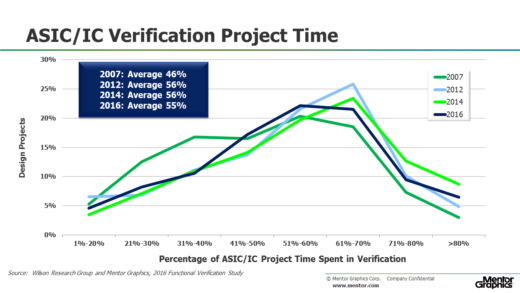
\includegraphics[width=0.8\linewidth]{images/wilson1.png}
  \caption{ASIC/IC项目中验证时间资源消耗统计}
  \label{fig:wilson_1}
\end{figure}

图\ref{fig:wilson_1}是来自Mentor的统计,展示了大部分的项目的验证时间均多于50\%,至于总体平均时间的略略缩短主要得益于近些年UVM技术的完善与成熟,这一点也是我们看中验证部分可以独立剥离的原因之一。

\begin{figure}
\centering
\begin{minipage}[t]{.5\textwidth}
  \centering
  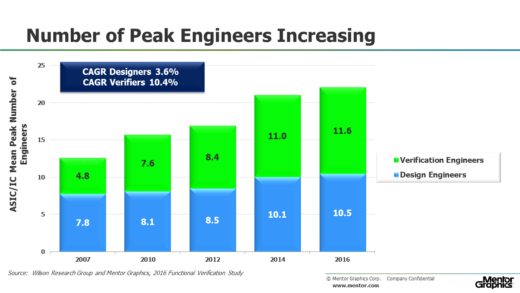
\includegraphics[width=0.95\linewidth]{images/wilson2.png}
  \captionof{figure}{设计/验证需求统计}
  \label{fig:wilson_2}
\end{minipage}%
\begin{minipage}[t]{.5\textwidth}
  \centering
  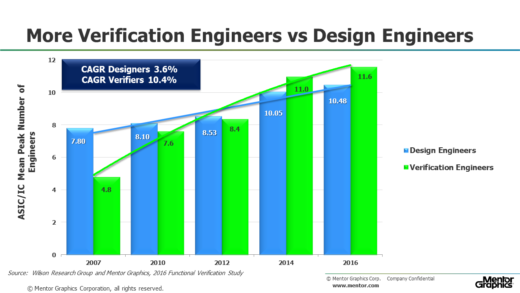
\includegraphics[width=0.95\linewidth]{images/wilson3.png}
  \captionof{figure}{设计/验证需求对比}
  \label{fig:wilson_3}
\end{minipage}
\end{figure}

图\ref{fig:wilson_2}与\ref{fig:wilson_3}展示了ASIC/IC设计与验证工程师的增长与对比,根据统计,项目中的验证需求明显愈发旺盛。

\begin{figure}[ht]
  \centering
  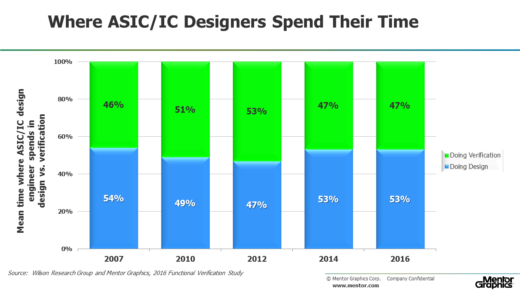
\includegraphics[width=0.8\linewidth]{images/wilson4.png}
  \caption{ASIC/IC项目中设计人员的时间消耗统计}
  \label{fig:wilson_4}
\end{figure}

图\ref{fig:wilson_4}说明,其实大部分设计人员也是有大概一半的时间在完成验证工作。

根据上图的统计,数字电路验证的需求是逐年不断增加的,主要原因有固化IP部分的复用导致设计人员的缩减,更主要的是ASIC工艺进步带来的SoC复杂性增加,为了减少流片风险,需要投入大量人力进入验证方向保证RTL的正确性(功能/行为/时序),在小公司火速增长的时代,芯片的生产周期缩短会带来抢占用户的先机,所以可以比竞争对手更快出芯片并且降低风险是所有芯片公司的目标,未来可预见fabless公司除了保留核心的算法之外,会将数字电路验证部分剥离出去,将主要资源集中在核心业务上,避免重复造轮子。

我们看到的是为所有半导体公司提供一个优质轮子的前景。

这一块业务在ASIC/IC领域起步较晚,在软件领域类比软件测试部分,已经有比较成熟的产业链,软件测试是一块比较特殊的软件项目过程,如果对软件要求比较高,则需要有软件测试部门控制质量,但是软件测试部门也有绩效,如果建在内部可能会在一些特定的质量问题上产生“纠缠”,如不客观、难以控制、测试人员与研发人员推诿责任的问题。最好的方法是委托专业的企业来负责测试部分,这样测试结果也客观,成本也得到控制,组织结构和决策方式也相对简单一点,一举多得。

ASIC数字验证有其相应的特点,知识体系范围较广,除了ASIC design相关知识之外,还需要UVM验证环境、SystemVerilog、OOP思想、linux、scripts、EDA仿真工具、常见的协议如AMBA、PCIE、USE、DDRARM/X86架构、低功耗UPF、混合仿真等等技术,相对于设计部分相对需要深度的技术面来说跨领域性较强、专业性要求更高,优秀的验证工程师更像是ASIC领域的软件工程师。对于fabless公司来说培养一个优秀的验证工程师的成本很高,但是同时需求又是如此强烈,所以类似软件测试的问题在ASIC部门也或多或少的存在,软件测试的独立委托需求的存在的合理性也同样适用在ASIC验证方向。

\begin{figure}[ht]
  \centering
  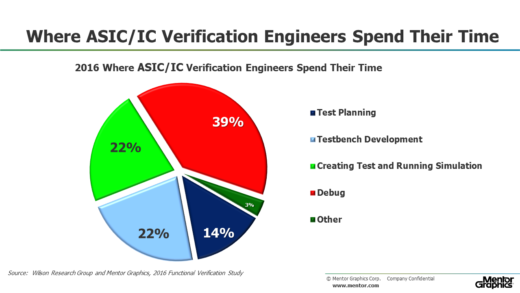
\includegraphics[width=0.8\linewidth]{images/wilson5.png}
  \caption{ASIC/IC项目中验证人员的时间消耗统计}
  \label{fig:wilson_5}
\end{figure}

图\ref{fig:wilson_5}展示了验证人员大部分的时间消耗在debug上面,其次是搭建TB与写case。Debug的时间消耗是根据case的情况决定的,基本无法提升效率,但是搭建TB与case的生成其实是可以实现自动化的。平台本质上是一个供ASIC流程运行的通用软件平台,可以基于B/S或C/S架构,在验证部分的应用是提供case生成、运行、coverage收集、regression等一系列流程的自动化,同时还可以将期间解析到的信息送到后台数据库,保留全部历史数据供后续的分析以及挖掘。平台的开发更偏软件一些,需要掌握数据库、client端开发、web端开发、browser端开发等互联网领域的知识,还需要掌握相应流程部分的知识,例如验证部分就是UVM、EDA仿真工具、混合仿真、c++/java/python软件开发等,对于知识体系的广度要求更高。利用上述平台,验证工程师的搭建TB与写case的工作可以实现复用,总体效率可以得到大幅度提升,预计在40\%左右。

那么我们利用“复用”的思路将验证需求独立出来,成立一个ASIC领域专业的第三方验证公司,统一由一批优秀的验证工程完成各个fabless公司委托。在公司内部,利用平台实现通用模块验证case的复用与数据统计,大幅提升效率,实现对ASIC验证产业的分工细化。

对于公司的服务模式类比软件测试服务模式,基于项目验证部分的一站式服务。项目规模不同,服务周期也不同,同时验证的时间节点会跟随客户项目的时间节点,所以按照目前市场的需求,预估大概服务费用会在50k/ppm,即每人每个月每个项目服务费用在50000¥左右,以年薪500000¥的验证工程师的能力,平均可以并行服务2-3个项目,再计算上平台的40\%的效率提升,在公司稳定阶段平均每人每年的服务费用在2100000¥左右。
\pagebreak

\section{行业竞争及市场渠道}
将ASIC验证独立出来是一块新兴业务,目前主营这类业务的公司比较少,有相关性的公司主要有:
\begin{enumerate}
\item 摩尔精英
  \begin{enumerate}
  \item 优点:
    \begin{enumerate}
    \item 初创公司更友好的服务,从咨询到招聘,从IT到委托;
    \item 近些年发展迅速。
    \end{enumerate}
  \item 缺点:
    \begin{enumerate}
    \item 经营业务过广;
    \item 目的不明确。
    \end{enumerate}
  \end{enumerate}
\item 芯原半导体 \& 灿芯半导体
  \begin{enumerate}
  \item 优点:
    \begin{enumerate}
    \item 一站式芯片设计服务;
    \item 国家集成电路基金战投;
    \item 进入ASIC服务行业较早,有一定规模效应。
    \end{enumerate}
  \item 缺点:
    \begin{enumerate}
    \item 主要面向大型客户或偏向后端客户;
    \item 无法满足对于RTL有保密需求的客户。
    \end{enumerate}
  \end{enumerate}
\item 创意电子 \& 世芯电子
  \begin{enumerate}
  \item 优点:
    \begin{enumerate}
    \item 专注于ASIC后端服务;
    \item 有优秀的客户资源。
    \end{enumerate}
  \item 缺点:
    \begin{enumerate}
    \item 台资背景;
    \item 前端服务市场发展缓慢。
    \end{enumerate}
  \end{enumerate}
\end{enumerate}

由于国内半导体产业基金的扶持以及AI的兴起,初创小公司的验证需求都比较强烈,因为这是除了核心设计之外的第一基本需求。在2017-2018年度,独自联系我们团队的验证委托任务的公司已经有四家。基于这块需求强烈的市场,我们前期的渠道主要有:
\begin{enumerate}
\item 项目周期要求高并且验证人手紧缺的初创小公司的SoC验证服务,有些公司有额外的平台需求,可以作为我们的另一项服务独立出来;
\item 发展中公司的平台需求;
\item 成熟公司的模块级验证需求。
\end{enumerate}

随着公司发展到成长期,规模在10人左右,可以在小公司拓展平台需求,因为平台可以大大优化所有验证工程师的效率,并利于习惯的养成;同时可以在发展中公司拓展SoC级验证需求,以及在成熟公司争取更多的模块级验证需求;当公司规模大于20人小于50人的时候,在维持小公司与发展中公司的验证需求的同时,主推平台需求,争取可以类比UVM一样成为ASIC验证方面的隐性标准平台,同时争取成熟公司的大规模验证需求。公司前中期的发展策略基本就是专注于验证领域以及推广验证平台。

当公司发展到稳定期的时候,规模大概在50-100人,这时可以根据市场容量考虑业务的纵向拓展还是横向拓展,策略上能植根于验证领域发掘出ASIC市场的更多验证需求比进入上下游领域有更高的优先级。

选择这样的策略主要是因为:
\begin{enumerate}
\item 大公司发展成熟,拥有自己的独立平台,如AMD的dj平台、NV的matrix平台,虽然都有各自的优缺点,而且平台不统一,但是验证工程师已经适应了各自的平台,所以渗透平台的可能性较低,但是模块众多,业务面广,很多模块有委托需求;
\item 发展中公司一般都可以独立完成相应项目的验证任务,但是平台发展不完善,验证效率较低,所以可以推广平台;
\item 创业小公司的验证人员紧缺,同时时效要求较高,可以同时主推第一需求验证服务的同时推广平台;
\item 平台前期渗透到后期推广,可以形成平台效应,有机会推广为隐性标准平台。
\end{enumerate}

验证委托公司的存在合理性是基于一条UNIX原则,Make each program do one thing well,一个程序做好一件事情,就是一家公司专注于一个领域,同时结合其它公司的专注领域来创造更多的价值。IDM垂直分工模式也是基于这样的思想,将验证领域继续细分出来之后,fabless公司专注于核心算法/架构设计,验证委托公司专注于RTL验证,后端委托公司专注与RTL2GDS的物理设计,制造厂与封测厂各司其知。

作为ASIC设计后续的第一需求阶段,验证委托公司同时可以在验证环境整合IP资源,降低集成IP的验证风险,同时可以考虑同后端委托公司合作完成除客户的核心设计外的一站式服务,通过公司的“复用”达到ASIC领域的资源利用最大化。
\pagebreak

\section{技术特点和核心竞争力}
能够做到高效的复用是提高验证效率的关键点之一:
\begin{enumerate}
\item 独立且完备的验证环境,利用OBTB原理构建一个可以被全部项目复用的验证环境;
\item 高复用性的验证用例以及验证序列,对于常见的协议可以做到完全复用;
\item 拥有完备的流程;
\item 可以提供白盒验证与黑盒(加密)验证服务;
\item 可以提供模块级与SoC级验证服务;
\item <more>
\end{enumerate}

能够利用平台自动化是关键点之二:
\begin{enumerate}
\item 验证用例、验证序列自动化生成;
\item 回归控制、回归自动化与数据收集;
\item 覆盖率自动化与收据收集;
\item <more>
\end{enumerate}

能够充分利用平台收集整理的数据是关键点之三:
\begin{enumerate}
\item 流程控制与数据解析;
\item 平台数据库设计与扩展;
\item 数据分析与验证风险提示;
\item 平台报告页面设计与应用;
\item <more>
\end{enumerate}

对于第一点,大部分公司可以做到其中的一部分,但是第二、第三点却少有公司能够充分利用,即使AMD、NV这种成熟公司,所以平台的充分利用会成为我们这一类验证委托公司的核心竞争力。
\pagebreak

\section{团队介绍}
衣冠宇:
\begin{enumerate}
\item 教育背景
  \begin{enumerate}
  \item 2009-2011 微电子学硕士 @ 荷兰代尔夫特理工大学
  \item 2005-2009 电子信息科学与工程 @ 南京大学
  \end{enumerate}
\item 科研背景
  \begin{enumerate}
  \item Compilation and Elaboration Speeding Up and Space Saving by Pre-Compilation, MSIE and Parallel Processing Technology
    \begin{enumerate}
    \item Guanyu Yi; Rosemary Hu; Gary Gao; etc.
    \item 2015年8月 CDNLive 上海,中国
    \end{enumerate}
  \item Towards a real-time high-definition depth sensor with hardware-efficient stereo matching
    \begin{enumerate}
    \item Ke Zhang; Guanyu Yi; C.-K. Liao; etc.
    \item 2012年2月 SPIE 圣地亚哥,美国
    \end{enumerate}
  \item Demo: Real-time depth extraction and viewpoint interpolation on FPGA
    \begin{enumerate}
    \item Guanyu Yi; Hsiu-Chi Yeh; Vanmeerbeeck, G.; etc.
    \item 2011年8月 ICDSC ACM/IEEE 根特,比利时
    \end{enumerate}
  \end{enumerate}
\item 工作背景
  \begin{enumerate}
  \item 2017/11 -- 现在~平台开发负责人 @ 世芯电子
  \item 2016/6 -- 2017/11 验证平台负责人 @ 中科院CPUxOS研究中心
  \item 2014/7 -- 2016/6 验证开发工程师 \& 平台开发工程师 @ 展讯通信
  \item 2011/9 -- 2014/7 验证工程师 @ AMD
  \end{enumerate}
\end{enumerate}

刘刚:
<more>

我们在大、中、小型公司历练过,一直致力于ASIC验证与平台技术的实现与推广,对于验证环境与平台的搭建与架构有自己的心得与成型产品。
<more>
\pagebreak

\section{融资计划和未来规划}
ASIC验证委托公司属于服务型公司,不直接面向产品,也无需直接承担流片风险,公司在市场需求充足的情况下亏损的风险很低。同时因为不需要流片,大大降低了公司的运营成本,可以快速实现收支平衡。公司的利润率主要是依靠高效的复用环境与平台来提升。

公司准备天使轮出20\%的股份融资5000000¥-10000000¥用于团队前期建设、服务器购置、办公场所租赁、人员招聘、市场营销等。预估平台与验证环境的磨合时间在6个月左右,同时第一年的公司影响力较弱的情况下,预计第一年公司的营业额在1000k-1500k之间,第二年公司运营会稳定很多,同时根据市场行情通过骨干员工招聘来完成验证效率最大化,争取达到收支平衡,第三年公司进入平稳发展期,根据市场行情考虑A轮出让15\%的股份扩大公司规模到10-20人,同时争取达到之前推算的2100000¥每人的公司年营业额。

公司的股权结构为:
\begin{enumerate}
\item 创始人 43\%
\item 联合创始人 42\%
\item 期权池 15\%
\end{enumerate}

公司的融资计划为:
\begin{enumerate}
\item 天使轮 20\%
\item A轮 15\%
\item B轮 10\%
\end{enumerate}

这样的股权结构及融资计划可以有如下几点保证:
\begin{enumerate}
\item 创始人对公司的绝对控制权;
\item 天使轮之后创始人对公司决策的一票否决权;
\item B轮之后还有C轮的裕量为上市做准备;
\item 联合创始人的参与最大化;
\end{enumerate}
\pagebreak



% \section{misc}
% \begin{figure}[ht]
%   \centering
%   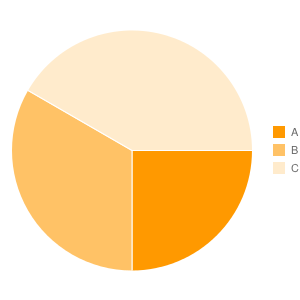
\includegraphics[width=5cm]{images/chart.png}
%   \caption{A chart}
%   \label{fig:chart}
% \end{figure}
% In Image \ref{fig:chart} you can see a chart.

% Operating figures of competition:
% \begin{center}
%   \begin{tabular}{l|l|r|r}
%     Company & Product & Price (\$) & \pbox{20cm}{Sales\\(Mio. \$)}\\
%     \hline
%     A & 1 & 100 & 1000\\
%     B\footnote{A footnote about B} & 2 & 100 & 1000\\
%     C & 3 & 100 & 1000\\
%   \end{tabular}
% \end{center}

% \begin{figure}
% \centering
% \begin{subfigure}{.5\textwidth}
%   \centering
%   
\includegraphics[width=.4\linewidth]{images/logo.png}
%   \caption{A subfigure}
%   \label{fig:sub1}
% \end{subfigure}%
% \begin{subfigure}{.5\textwidth}
%   \centering
%   
\includegraphics[width=.4\linewidth]{images/logo.png}
%   \caption{A subfigure}
%   \label{fig:sub2}
% \end{subfigure}
% \caption{A figure with two subfigures}
% \label{fig:test}
% \end{figure}

% \begin{figure}
% \centering
% \begin{minipage}{.5\textwidth}
%   \centering
%   
\includegraphics[width=.4\linewidth]{images/logo.png}
%   \captionof{figure}{A figure}
%   \label{fig:test1}
% \end{minipage}%
% \begin{minipage}{.5\textwidth}
%   \centering
%   
\includegraphics[width=.4\linewidth]{images/logo.png}
%   \captionof{figure}{Another figure}
%   \label{fig:test2}
% \end{minipage}
% \end{figure}

\clearpage
\end{document}

%%% Local Variables:
%%% mode: xetex
%%% TeX-master: t
%%% End:
